\documentclass{math}

\usepackage{circuitikz}
\usepackage{tikz}

\title{University Physics 2}
\author{Alvin Lin}
\date{January 2018 - May 2018}

\begin{document}

\maketitle

\section*{Capacitors}
Capacitors are represented usually as two parallel plates.
\begin{center}
  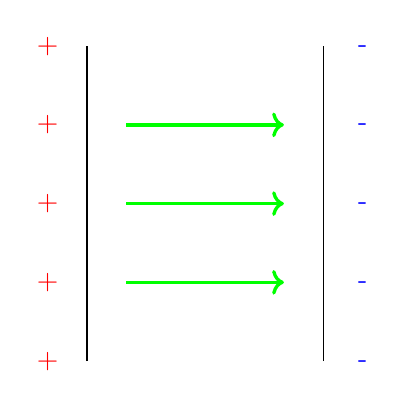
\begin{tikzpicture}
    \draw (0,0) -- (0,4);
    \draw[->,green,very thick] (0.5,1) -- (2.5,1);
    \draw[->,green,very thick] (0.5,2) -- (2.5,2);
    \draw[->,green,very thick] (0.5,3) -- (2.5,3);
    \draw (3,0) -- (3,4);
    \foreach \y in {0,1,2,3,4} {
      \node[red] at (-0.5,\y) {+};
      \node[blue] at (3.5,\y) {-};
    }
  \end{tikzpicture}
\end{center}
\[ E = \frac{\sigma}{\epsilon_{\circ}} \]
\[ \Delta V = -\int_{0}^{d}\vec{E}\cdot\diff{\vec{x}} =
  -\int_{0}^{d}\frac{\sigma}{\epsilon_{\circ}}\diff{x} \]
Capacitance is defined as:
\[ C \equiv \bigg|\frac{Q}{\Delta V}\bigg| \]
Capacitance is measured in units of Farads, equivalent to Coulombs over
volts. For parallel plates:
\[ C = \frac{Q}{\Delta V} = \frac{Q}{\frac{Qd}{A\epsilon_{\circ}}} =
  \frac{A\epsilon_{\circ}}{d} \]
The assumes you have a vacuum between plates, generally this is not the case as
there is some insulating material between the plates. Different materials
determine the properties of the capacitor. Capacitance for this is:
\[ C = C_{\circ}\kappa = \kappa\epsilon_{\circ}\frac{A}{d} =
  \epsilon\frac{A}{d} \]
where \( \kappa \) is the dielectric constant. \( \kappa\epsilon_{\circ} \) is
the permitivity of whatever material is used, and both constants are properties
of the material. \( \kappa \) is always greater than 1, with \( \kappa = 1 \)
being the dielectric constant for a vacuum.

\subsection*{Capacitors in Series}
\begin{center}
  \begin{circuitikz}
    \draw (0,0) to[battery, l=\( \Delta V \)] (0,4) -- (4,4)
      to[capacitor, l=\( C_1 \)] (4,2)
      to[capacitor, l=\( C_2 \)] (4,0) -- (0,0);
  \end{circuitikz}
\end{center}
Both \( C_1 \) and \( C_2 \) have the same charge \( Q \) due to being in series
with the battery.
\[ Q_1 = Q_2 = Q \quad C_1 = \frac{Q}{\Delta V_1} \quad
  C_2 = \frac{Q}{\Delta V_2} \]
By conservation of energy, we know that:
\begin{align*}
  |\Delta V_{total}| &= \Delta V_1+\Delta V_2 \\
  C_{eq} &= \frac{Q}{\Delta V_{total}} \\
  Q &= C_{eq}(\Delta V_1+\Delta V_2) \\
  Q &= C_{eq}(\frac{Q}{C_1}+\frac{Q}{C_2}) \\
  \frac{1}{C_{eq}} &= \frac{1}{C_1}+\frac{1}{C_2}
\end{align*}

\subsection*{Capacitors in Parallel}
\begin{center}
  \begin{circuitikz}
    \draw (0,0) to[battery, l=\( \Delta V \)] (0,4) -- (4,4)
      to[capacitor, l=\( C_1 \)] (4,0) -- (0,0);
    \draw (4,4) -- (8,4)
      to[capacitor, l=\( C_2 \)] (8,0) -- (4,0);
  \end{circuitikz}
\end{center}
By conservation of charge:
\[ Q = Q_1+Q_2 \]
We can simplify this circuit to:
\begin{center}
  \begin{circuitikz}
    \draw (0,0) to[battery, l=\( \Delta V \)] (0,4) -- (4,4)
      to[capacitor, l=\( C_{eq} \)] (4,0) -- (0,0);
  \end{circuitikz}
\end{center}
By conservation of energy:
\begin{align*}
  \Delta V_1 &= \Delta V \\
  \Delta V_2 &= \Delta V \\
  C_{eq} &= \frac{Q}{\Delta V} \\
  &= \frac{Q_1+Q_2}{\Delta V} \\
  &= \frac{Q_1}{\Delta V}+\frac{Q_2}{\Delta V} \\
  &= C_1+C_2
\end{align*}

\subsection*{Energy in a Capacitor}
To find the energy in a capacitor, find the work needed to charge it. Recall:
\[ C = \frac{Q}{V} \]
Suppose it is partially charged:
\[ V = \frac{q}{C} \quad \diff{V} = \frac{\diff{q}}{C} \]
where \( V \) is the intermediate voltage and \( q \) is the intermediate
charge.
\begin{align*}
  W &= \int\vec{F}\cdot\diff{\vec{r}} \\
  \diff{W} &= \vec{F}\cdot\diff{\vec{r}} \\
  V &= -\int\vec{E}\cdot\diff{\vec{r}} \\
  \diff{V} &= |\vec{E}|\diff{r} \\
  \diff{W} &= F\diff{r} = (q|\vec{E}|)\diff{r} = q\diff{V} \\
  W &= \int q\diff{V} = \int_{0}^{Q}q(\frac{\diff{q}}{c}) = \frac{Q^2}{2C}
\end{align*}
As a relation to the equations for voltage:
\[ U = \frac{Q^2}{2C} = \frac{1}{2}CV^2 = \frac{1}{2}QV \]
If we want energy density as energy over volume:
\begin{align*}
  u &= \frac{U}{volume} \\
  &= \frac{\frac{1}{2}CV^2}{Ad} \\
  &= \frac{\frac{1}{2}(\frac{\epsilon_{\circ}A}{d})(Ed)^2}{Ad} \\
  &= \frac{1}{2}\epsilon_{\circ}E^2
\end{align*}

\begin{center}
  You can find all my notes at \url{http://omgimanerd.tech/notes}. If you have
  any questions, comments, or concerns, please contact me at
  alvin@omgimanerd.tech
\end{center}

\end{document}
